% =============================================================================
% Autore originale: Fabio Tempera
% Licenza: MIT (vedere LICENSE nel medesimo direttorio)
%
% DOCUMENTO
%   Template interno CieloBuio OdV per il resoconto di selezione dei siti
%   candidati di una rete regionale TESS-4C. Questo esemplare è compilato
%   sull'Abruzzo (20 nodi, metodo già usato in Umbria). Non destinato
%   a scuole, parchi o atenei: la lettera verso gli enti resta il file separato
%   template_TESS4C_CieloBuio.
%
% COME RIUSARLO IN UN'ALTRA REGIONE
%   Sostituire toponimi, coordinate, letture VIIRS, popolazione e quote;
%   aggiornare le figure in figures/ (mappa e grafico di radianza in SVG e
%   PNG ad alta risoluzione). Lasciare invariati preambolo sull'inquinamento
%   luminoso, sezione sull'osservabile e criteri di installazione.
%
% COMPILAZIONE
%   pdflatex resoconto-abruzzo.tex  (due passate per i riferimenti a Figure e Tabelle)
%   Classe report, pacchetti in packages.sty. Non usare Markdown.
% =============================================================================

\documentclass[11pt,a4paper]{report}

\usepackage{packages}

\definecolor{nightblue}{RGB}{22,38,58}
\definecolor{steel}{RGB}{80,100,120}
\definecolor{linegray}{RGB}{200,200,200}

\renewcommand{\thesection}{\arabic{section}}
\renewcommand{\thefigure}{\arabic{figure}}
\renewcommand{\thetable}{\arabic{table}}
\setcounter{secnumdepth}{0}

\titleformat{\section}
  {\normalfont\Large\bfseries\color{nightblue}}
  {\thesection}{0.6em}{}
\titleformat{\subsection}
  {\normalfont\large\bfseries\color{nightblue}}
  {\thesubsection}{0.6em}{}
\titlespacing{\section}{0pt}{1.4em}{0.6em}
\titlespacing{\subsection}{0pt}{1.1em}{0.4em}

\pagestyle{fancy}
\fancyhf{}
\renewcommand{\headrulewidth}{0.4pt}
\renewcommand{\headrule}{\hbox to\headwidth{\color{linegray}\leaders\hrule height \headrulewidth\hfill}}
\fancyhead[L]{\small\color{steel} CieloBuio OdV, uso interno}
\fancyhead[R]{\small\color{steel} Siti candidati TESS-4C Abruzzo}
\fancyfoot[C]{\small\color{steel}\thepage}

\hyphenation{Avezzano}
\hypersetup{
  colorlinks=true,
  linkcolor=nightblue,
  urlcolor=nightblue,
  citecolor=nightblue,
  pdftitle={Resoconto della selezione dei siti candidati. Rete regionale TESS-4C Abruzzo},
  pdfauthor={Fabio Tempera}
}

\setlist[itemize]{leftmargin=1.4em, itemsep=0.25em, topsep=0.3em}
\setlist[enumerate]{leftmargin=1.6em, itemsep=0.25em, topsep=0.3em}

\newcommand{\infobox}[1]{%

  \begin{center}

  \renewcommand{\arraystretch}{1.5}

  \begin{tabularx}{\linewidth}{X}
    \arrayrulecolor{linegray}
    \toprule
    #1 \\
    \bottomrule
  \end{tabularx}

  \end{center}

}

\begin{document}

\begin{center}

{\LARGE\bfseries\color{nightblue} 20 siti candidati per la rete regionale di fotometri TESS-4C in Abruzzo\par}

\vspace{0.2cm}

{\large Resoconto della selezione\par}

\vspace{0.1cm}

{\small CieloBuio OdV, progetto rete regionale TESS-4C\par}

{\small Documento interno, non destinato a scuole, parchi o atenei.}

\end{center}

% Uso interno CieloBuio. I 20 nodi restano fuori dalla lettera agli enti.
\section*{Oggetto}
\addcontentsline{toc}{section}{Oggetto}

Il presente resoconto fissa i 20 siti candidati della rete regionale abruzzese di monitoraggio della qualità del cielo notturno con fotometri \textit{TESS-4C}. La rete si inserisce nel progetto nazionale coordinato da CieloBuio OdV. Il metodo è quello già applicato in Umbria: circa 20 nodi per regione, distribuiti sulle tipologie territoriali e verificati sullo strato satellitare \textit{VIIRS} più recente, in modo da coprire l'intervallo di radianza misurato sul territorio.

Il testo è scritto per il gruppo, non tutti i soci sono astronomici di professione. Per questo, prima dell'elenco dei siti, si richiamano l'osservabile, la differenza tra satellite e terra, l'aspetto dello strumento e i vincoli di installazione. La lettera da inviare a scuole, parchi e atenei è un documento separato (template nazionale) e \textit{non} include questa lista.

\infobox{%
\textit{In sintesi}: 20 nodi, tutti in Abruzzo, sulle 4 province; 8 categorie territoriali coperte; radianza VIIRS 2025 da 0,000 a 95,360 nW\,cm$^{-2}$\,sr$^{-1}$; coordinate WGS84, popolazione Istat al 1 gennaio 2026, quota del pixel Copernicus WorldDEM-30.
}

\section*{L'inquinamento luminoso}
\addcontentsline{toc}{section}{L'inquinamento luminoso}

L'inquinamento luminoso è un problema globale che, al pari di altre forme di inquinamento di origine antropica, produce effetti sugli ecosistemi e sugli organismi viventi. Il dibattito è nato nella comunità astronomica professionale, preoccupata che l'uso inefficiente, superfluo e non controllato della luce artificiale notturna (\textit{artificial light at night}, ALAN) potesse compromettere la visibilità del cielo stellato dagli osservatori. Oggi lo stesso fenomeno è oggetto di ricerca interdisciplinare, di studi socioeconomici e di un dibattito culturale sul cielo notturno come patrimonio.

Gli effetti della luce artificiale notturna sono legati allo sviluppo e all'uso improprio di sorgenti sempre più efficienti e spesso più economiche. Negli anni 70 la transizione in discussione era quella dalle lampade al mercurio a quelle al sodio ad alta pressione. Oggi è in corso un passaggio verso i diodi a emissione di luce (LED). La distribuzione spettrale di potenza è cambiata: da poche righe di emissione si è passati a un numero elevato di componenti, con un continuo più intenso soprattutto nel blu e nel verde.

A questa transizione si accompagna un aumento della luce artificiale a quasi tutte le scale spaziali. Si stima che circa il 99\% della popolazione di Stati Uniti ed Europa viva sotto un cielo inquinato, e che più del 33\% della popolazione mondiale non possa più osservare la Via Lattea (Falchi et al., 2016). Nemmeno le aree remote sono immuni: la luce artificiale si propaga nell'atmosfera e produce un alone visibile a grande distanza dalla sorgente.

I dati oggettivi e accessibili sono la base per qualsiasi norma di mitigazione e per misurarne l'efficacia. In Italia diverse regioni dispongono di leggi sul contenimento della luce artificiale. In assenza di reti di misura a terra, il monitoraggio si appoggia spesso a stime satellitari, poco puntuali rispetto a una stazione in sito. Il progetto CieloBuio propone una rete di stazioni su base volontaria in tutte le regioni.

Il preambolo di questa sezione è stato riadattato da rassegne e articoli di riferimento sulla luce artificiale notturna, in particolare Chepesiuk (2009), Bennie et al.\ (2015), Irwin (2018), Svechkina et al.\ (2020), Walker (1970), Riegel (1973), DiLaura (2008), Kyba et al.\ (2017 e 2023), Sánchez de Miguel et al.\ (2021) e Falchi et al.\ (2016). Per lo strumento TESS il riferimento tecnico è Zamorano et al.\ (2016); per il Day/Night Band di VIIRS, Liao et al.\ (2013). L'elenco bibliografico esteso non viene riportato, per non appesantire un testo destinato a un uso operativo.

\section*{Cosa si misura}
\addcontentsline{toc}{section}{Cosa si misura}

Il fotometro \textit{non} misura l'inquinamento luminoso. Lo strumento misura una brillanza superficiale del cielo (candele per metro quadro, oppure magnitudini per arcosecondo quadro in una banda). Quel numero è la somma di un contributo naturale (stelle, polvere interstellare, luce zodiacale, airglow) e di un contributo artificiale. Interpretare i dati, e separare le 2 componenti, è il lavoro dell'esperto.

Lo strato VIIRS, usato per scegliere i siti, è un altro osservabile: radianza notturna uscente verso il satellite, in nW\,cm$^{-2}$\,sr$^{-1}$. La radianza satellitare indica dove il territorio è acceso e dove è buio, e non coincide con la brillanza zenitale che registrerà il TESS-4C. Per questo, accanto alle tabelle, il resoconto usa mappa e grafici a colori.

La Figura~\ref{fig:contributi} schematizza la somma dei 2 contributi.

\begin{figure}[ht!]
\centering
% Figura: scripts/generate_contributi.py (repo tess4c-figure-scripts). Schema didattico nello script, non un JSON.
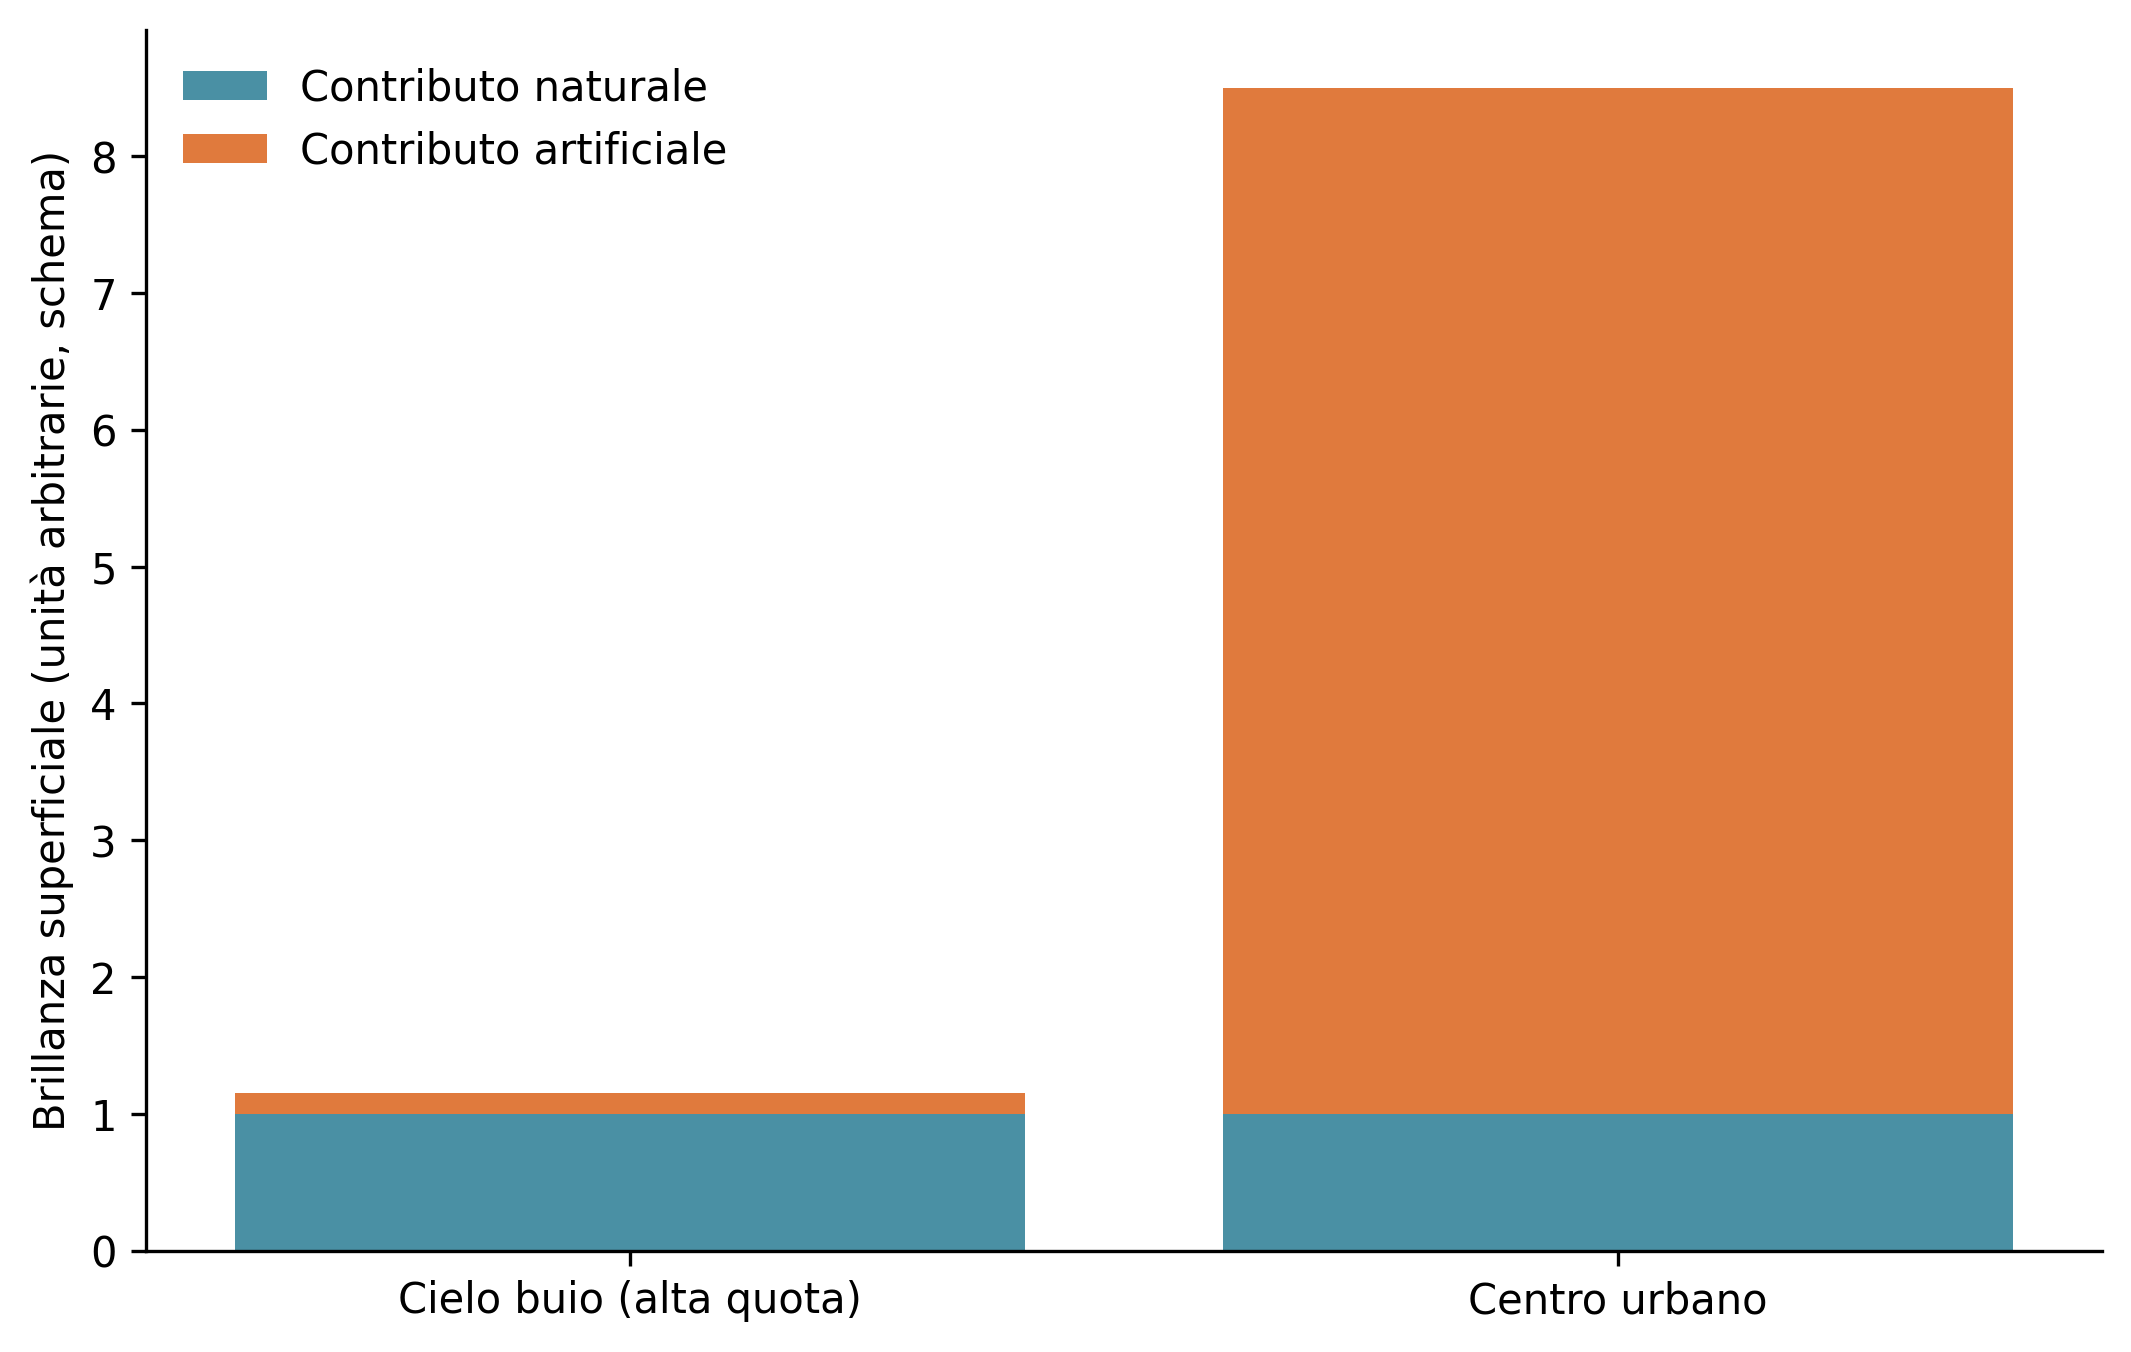
\includegraphics[width=0.92\textwidth]{figures/contributi_brillanza.png}
\caption{Schema della brillanza superficiale come somma di contributo naturale e artificiale. Barre illustrative, non misure abruzzesi.}
\label{fig:contributi}
\end{figure}

\section*{Lo strumento e l'installazione}
\addcontentsline{toc}{section}{Lo strumento e l'installazione}

Lo strumento previsto è il TESS-4C, evoluzione a 4 bande del TESS-W (GUAIX, Universidad Complutense de Madrid, progetto STARS4ALL). Lo strumento è alloggiato in un contenitore stagno dell'ordine di 87$\times$75$\times$45\,mm, con alimentazione 5\,V USB, WiFi e protocollo \texttt{MQTT}. Lo strumento non è una cupola da osservatorio. La Figura~\ref{fig:tessw} e la Figura~\ref{fig:tess4c} mostrano l'aspetto reale e le 4 bande.

\begin{figure}[ht!]
\centering
% Immagine ufficiale STARS4ALL / GUAIX-UCM. Non generata dagli script di figura.
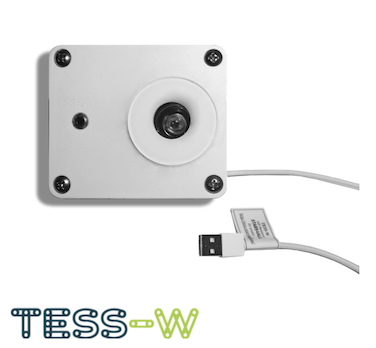
\includegraphics[width=0.55\textwidth]{figures/tess-w.png}
\caption{Fotometro TESS-W in contenitore stagno. Immagine ufficiale STARS4ALL / GUAIX-UCM.}
\label{fig:tessw}
\end{figure}

\begin{figure}[ht!]
\centering
% Immagine ufficiale GUAIX-UCM. Non generata dagli script di figura.
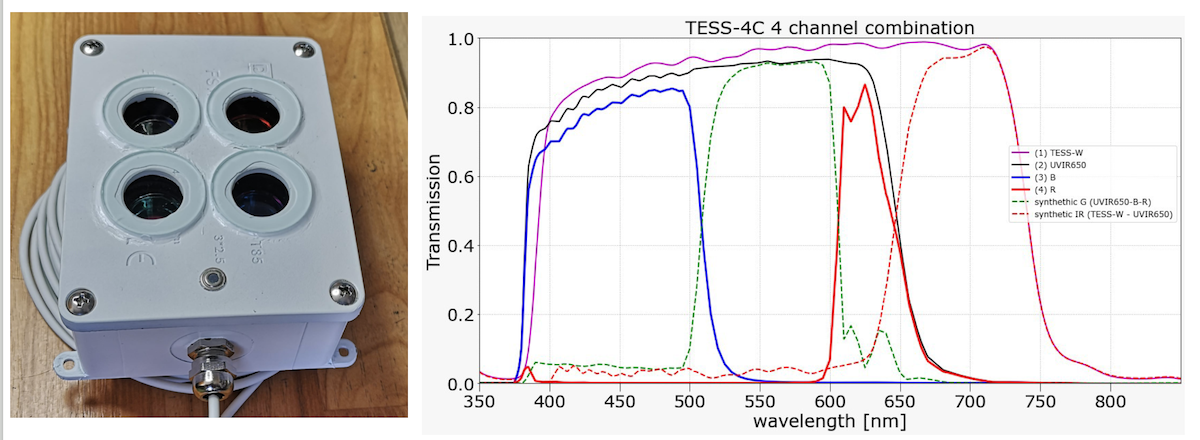
\includegraphics[width=\textwidth]{figures/tess-4c.png}
\caption{TESS-4C e curve di risposta dei 4 canali. Fonte: GUAIX-UCM.}
\label{fig:tess4c}
\end{figure}

Prima di confermare un nodo, un sopralluogo notturno resta necessario. Se un lampione, un'insegna o un faro di sicurezza entra nel campo di vista (circa 17$^{\circ}$), lo strumento misura quella luce, non il cielo. Il sito deve disporre anche di corrente e di WiFi, oppure di un modulo dati nei rifugi.

La Figura~\ref{fig:installazione} confronta le 2 geometrie da verificare in situ. A sinistra il fotometro è sul cornicione, esposto al lampione: un raggio diretto raggiunge l'ottica, il campo di vista verso lo zenit risulta contaminato e lo strumento registra la sorgente, non il cielo. A destra il fotometro è al centro del tetto, lontano dal bordo, con zenit libero; il lampione resta sotto il piano di falda e l'edificio lo scherma. L'alimentazione a 5\,V e la copertura WiFi restano necessarie, anche se non sono indicate nel disegno.

\begin{figure}[ht!]
\centering

\begin{tabular}{@{}cc@{}}
% Illustrazioni fisse di posa. Non generate dagli script di figura.
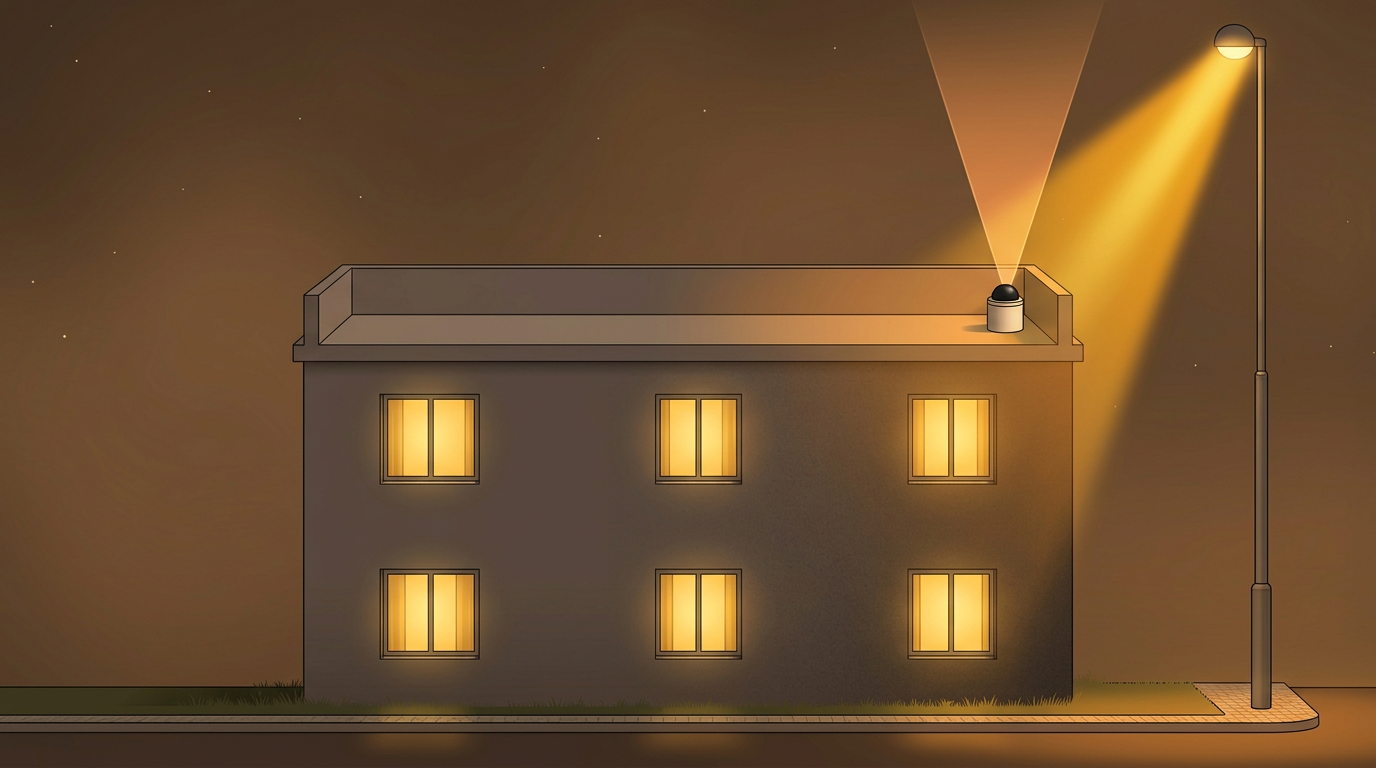
\includegraphics[width=0.48\textwidth]{figures/installazione_non_idonea.png} &
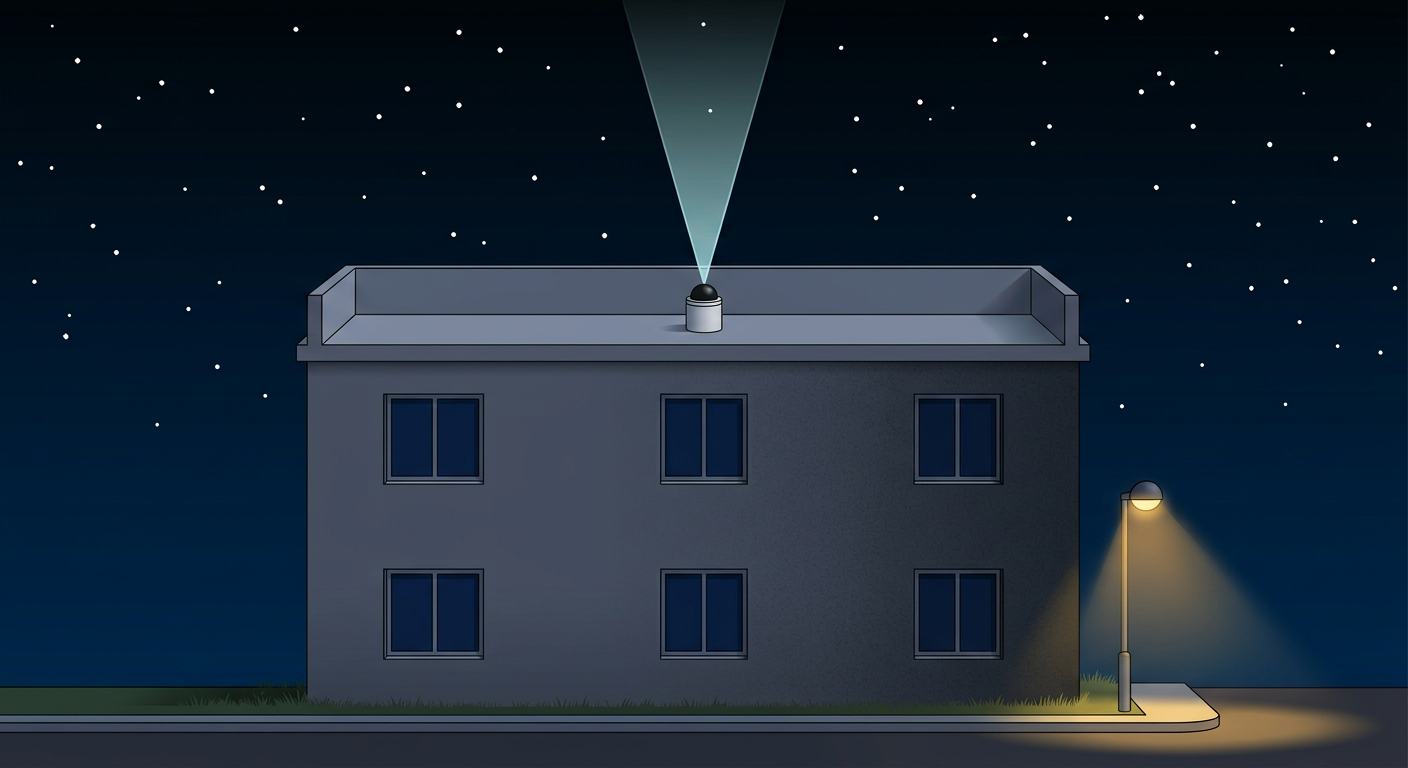
\includegraphics[width=0.48\textwidth]{figures/installazione_idonea.png}
\end{tabular}

\caption{Installazione del fotometro: geometria non idonea (sinistra) e geometria idonea (destra).}
\label{fig:installazione}
\end{figure}

I 2 siti scientifici (Campo Imperatore e Collurania) restano candidati e vanno confermati; la rete procede comunque.

\section*{Criteri}
\addcontentsline{toc}{section}{Criteri}

Ogni nodo è interno ai confini amministrativi delle province dell'Aquila, Teramo, Pescara e Chieti. Le coordinate sono in WGS84. Per i centri abitati si usano le coordinate geodetiche di Wikipedia del comune o della piazza di riferimento. Per Atessa si usano le coordinate della casa comunale pubblicate da Tuttitalia, perché la voce Wikipedia del comune riporta le coordinate solo in gradi e primi. Per Caramanico Terme si usano le coordinate OpenStreetMap. Per gli osservatori e il Rifugio Bruno Pomilio si usano le coordinate delle voci Wikipedia dedicate.

La radianza è letta in modo puntuale su \url{https://www.lightpollutionmap.info/}, strato \textit{VIIRS} 2025 (NASA Black Marble VJ146A4, composito annuale AllAngle Composite Snow Free). L'unità è nW\,cm$^{-2}$\,sr$^{-1}$. Il prodotto NASA pone a 0 i pixel inferiori a 0,5 nW\,cm$^{-2}$\,sr$^{-1}$: il valore 0,000 è la lettura dello strumento. Lo strato 2025 è l'annualità più recente disponibile al momento dello studio (help del servizio aggiornato al 30 giugno 2026). La quota riportata è quella del pixel campionato (Copernicus WorldDEM-30), restituita dallo stesso strumento. La popolazione è quella Istat dei residenti al 1 gennaio 2026, via Tuttitalia.

Le 8 categorie sono: centro urbano grande (oltre 40.000 abitanti), centro urbano medio (da 10.000 a 40.000), centro urbano piccolo o borgo, costa, collina interna, montagna o alta quota, area protetta o parco, sito scientifico di riferimento. Vasto supera i 40.000 abitanti e resta assegnato alla costa, perché rappresenta il litorale sud-orientale della provincia di Chieti; i centri urbani grandi sono già coperti da Pescara, L'Aquila e Avezzano.

% Mappa e grafico: SVG e PNG ad alta risoluzione in figures/.
\section*{I 20 siti}
\addcontentsline{toc}{section}{I 20 siti}

La Figura~\ref{fig:mappa} colloca i 20 nodi sulle coordinate usate per la lettura \textit{VIIRS}. I numeri coincidono con la colonna n.\ delle tabelle successive.

\begin{figure}[ht!]
\centering
% Figura: scripts/generate_map.py (repo tess4c-figure-scripts). Dati: data/sites.json (chiavi sites e map).
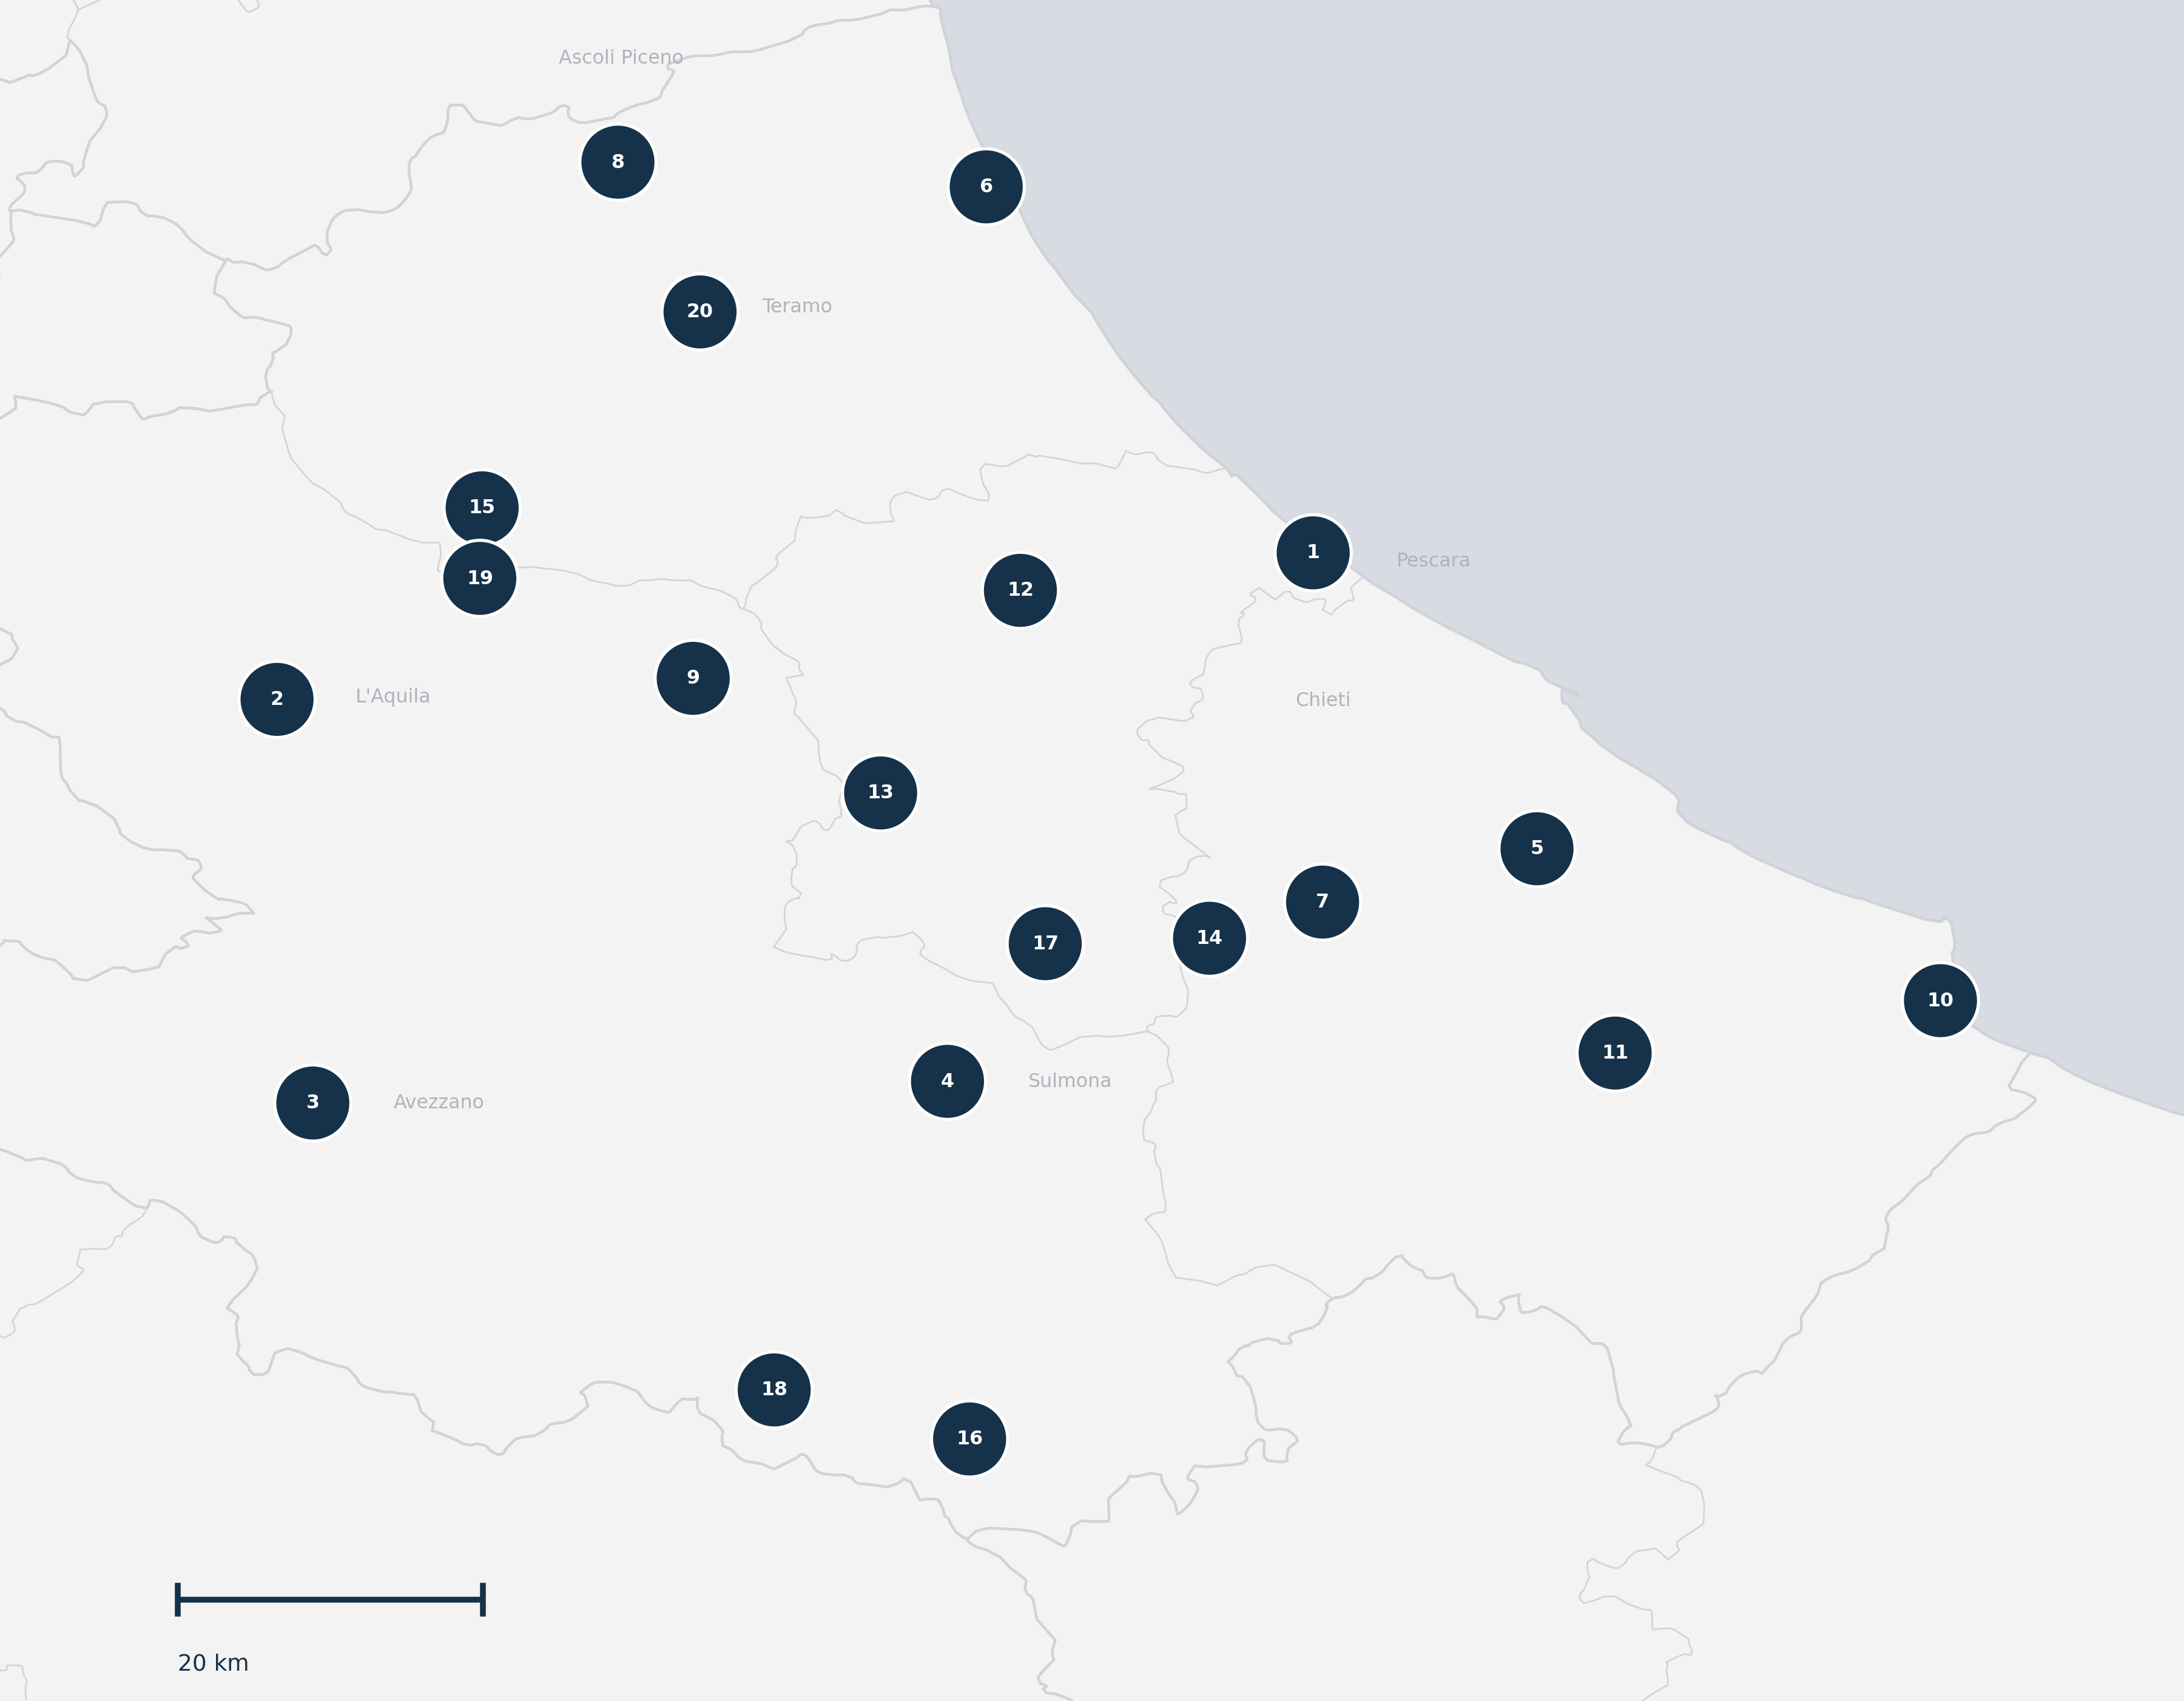
\includegraphics[width=\textwidth]{figures/mappa_siti_TESS4C_Abruzzo.png}
\caption{I 20 siti candidati della rete TESS-4C Abruzzo. Punti in WGS84 su confini amministrativi italiani.}
\label{fig:mappa}
\end{figure}

\FloatBarrier

La Tabella~\ref{tab:anagrafica} riporta categoria, comune e coordinate. La Tabella~\ref{tab:misure} riporta quota del pixel, popolazione comunale e radianza \textit{VIIRS} 2025.

\begin{table}[ht!]
\centering
\renewcommand{\arraystretch}{1.5}
\setlength{\tabcolsep}{3.4pt}
\small

\begin{tabular}{@{}r l l l r r@{}}
\toprule
n. & Nome & Categoria & Comune (prov.) & Lat N & Lon E \\
\midrule
1 & Pescara, centro & urbano grande & Pescara (PE) & 42,464278 & 14,214189 \\
2 & L'Aquila, Duomo & urbano grande & L'Aquila (AQ) & 42,348870 & 13,398180 \\
3 & Avezzano & urbano grande & Avezzano (AQ) & 42,030975 & 13,426372 \\
4 & Sulmona & urbano medio & Sulmona (AQ) & 42,048025 & 13,926198 \\
5 & Lanciano & urbano medio & Lanciano (CH) & 42,231211 & 14,390472 \\
6 & Giulianova & urbano medio & Giulianova (TE) & 42,752517 & 13,956686 \\
7 & Guardiagrele & urbano piccolo & Guardiagrele (CH) & 42,189222 & 14,221592 \\
8 & Civitella del Tronto & urbano piccolo & Civitella del Tronto (TE) & 42,771944 & 13,666667 \\
9 & Castel del Monte & urbano piccolo & Castel del Monte (AQ) & 42,365440 & 13,725920 \\
10 & Vasto, centro & costa & Vasto (CH) & 42,111589 & 14,708219 \\
11 & Atessa & collina interna & Atessa (CH) & 42,070300 & 14,452000 \\
12 & Loreto Aprutino & collina interna & Loreto Aprutino (PE) & 42,434722 & 13,983611 \\
13 & Corvara & collina interna & Corvara (PE) & 42,275171 & 13,873535 \\
14 & Rifugio Bruno Pomilio & montagna & Rapino (CH) & 42,160736 & 14,132572 \\
15 & Prati di Tivo & montagna & Pietracamela (TE) & 42,499722 & 13,559722 \\
16 & Civitella Alfedena & area protetta & Civitella Alfedena (AQ) & 41,766389 & 13,943611 \\
17 & Caramanico Terme & area protetta & Caramanico Terme (PE) & 42,156446 & 14,003189 \\
18 & Pescasseroli & area protetta & Pescasseroli (AQ) & 41,805000 & 13,789722 \\
19 & Campo Imperatore & sito scientifico & L'Aquila (AQ) & 42,444158 & 13,557875 \\
20 & Collurania & sito scientifico & Teramo (TE) & 42,654025 & 13,731322 \\
\bottomrule
\end{tabular}

\caption{Anagrafica dei 20 siti candidati. Coordinate WGS84 del punto di lettura VIIRS.}
\label{tab:anagrafica}
\end{table}

\FloatBarrier

\begin{table}[ht!]
\centering
\renewcommand{\arraystretch}{1.5}
\small

\begin{tabular}{@{}r l r r r@{}}
\toprule
n. & Nome & Quota (m) & Popolazione & VIIRS 2025 \\
\midrule
1 & Pescara, centro & 19 & 118.487 & 94,044 \\
2 & L'Aquila, Piazza del Duomo & 717 & 70.803 & 95,360 \\
3 & Avezzano & 689 & 41.238 & 46,795 \\
4 & Sulmona & 399 & 21.610 & 57,356 \\
5 & Lanciano & 272 & 33.843 & 37,754 \\
6 & Giulianova & 70 & 23.556 & 34,295 \\
7 & Guardiagrele & 591 & 8.161 & 15,008 \\
8 & Civitella del Tronto & 585 & 4.555 & 8,304 \\
9 & Castel del Monte & 1.336 & 379 & 20,408 \\
10 & Vasto, centro & 150 & 40.920 & 75,646 \\
11 & Atessa & 403 & 10.208 & 16,736 \\
12 & Loreto Aprutino & 261 & 7.037 & 28,574 \\
13 & Corvara & 631 & 186 & 2,360 \\
14 & Rifugio Bruno Pomilio & 1.894 & n.d. & 0,000 \\
15 & Prati di Tivo & 1.451 & 196 & 2,338 \\
16 & Civitella Alfedena & 1.083 & 287 & 6,084 \\
17 & Caramanico Terme & 603 & 1.703 & 16,854 \\
18 & Pescasseroli & 1.145 & 1.993 & 12,972 \\
19 & Campo Imperatore & 2.147 & n.d. & 0,000 \\
20 & Collurania & 396 & n.d. & 3,018 \\
\bottomrule
\end{tabular}

\caption{Misure dei 20 siti. Popolazione: residenti Istat al 1 gennaio 2026 del comune. Quota: metro sul livello del mare del pixel VIIRS (Copernicus WorldDEM-30). Radianza: VIIRS 2025 in nW\,cm$^{-2}$\,sr$^{-1}$.}
\label{tab:misure}
\end{table}

\FloatBarrier

La Tabella~\ref{tab:categorie} e la Figura~\ref{fig:categorie} riepilogano l'assegnazione alle 8 categorie. La Figura~\ref{fig:province} mostra i nodi per provincia.

\begin{table}[ht!]
\centering
\renewcommand{\arraystretch}{1.5}

\begin{tabularx}{\linewidth}{@{}l X@{}}
\toprule
Categoria & Nodi \\
\midrule
Centro urbano grande & 1 Pescara, 2 L'Aquila, 3 Avezzano \\
Centro urbano medio & 4 Sulmona, 5 Lanciano, 6 Giulianova \\
Centro urbano piccolo / borgo & 7 Guardiagrele, 8 Civitella del Tronto, 9 Castel del Monte \\
Costa & 10 Vasto \\
Collina interna & 11 Atessa, 12 Loreto Aprutino, 13 Corvara (PE) \\
Montagna / alta quota & 14 Rifugio Bruno Pomilio, 15 Prati di Tivo \\
Area protetta / parco & 16 Civitella Alfedena, 17 Caramanico Terme, 18 Pescasseroli \\
Sito scientifico di riferimento & 19 Campo Imperatore, 20 Collurania \\
\bottomrule
\end{tabularx}

\caption{Copertura delle 8 categorie territoriali.}
\label{tab:categorie}
\end{table}

\begin{figure}[ht!]
\centering
% Figura: scripts/generate_categorie.py (repo tess4c-figure-scripts). Dati: data/sites.json, campo category.
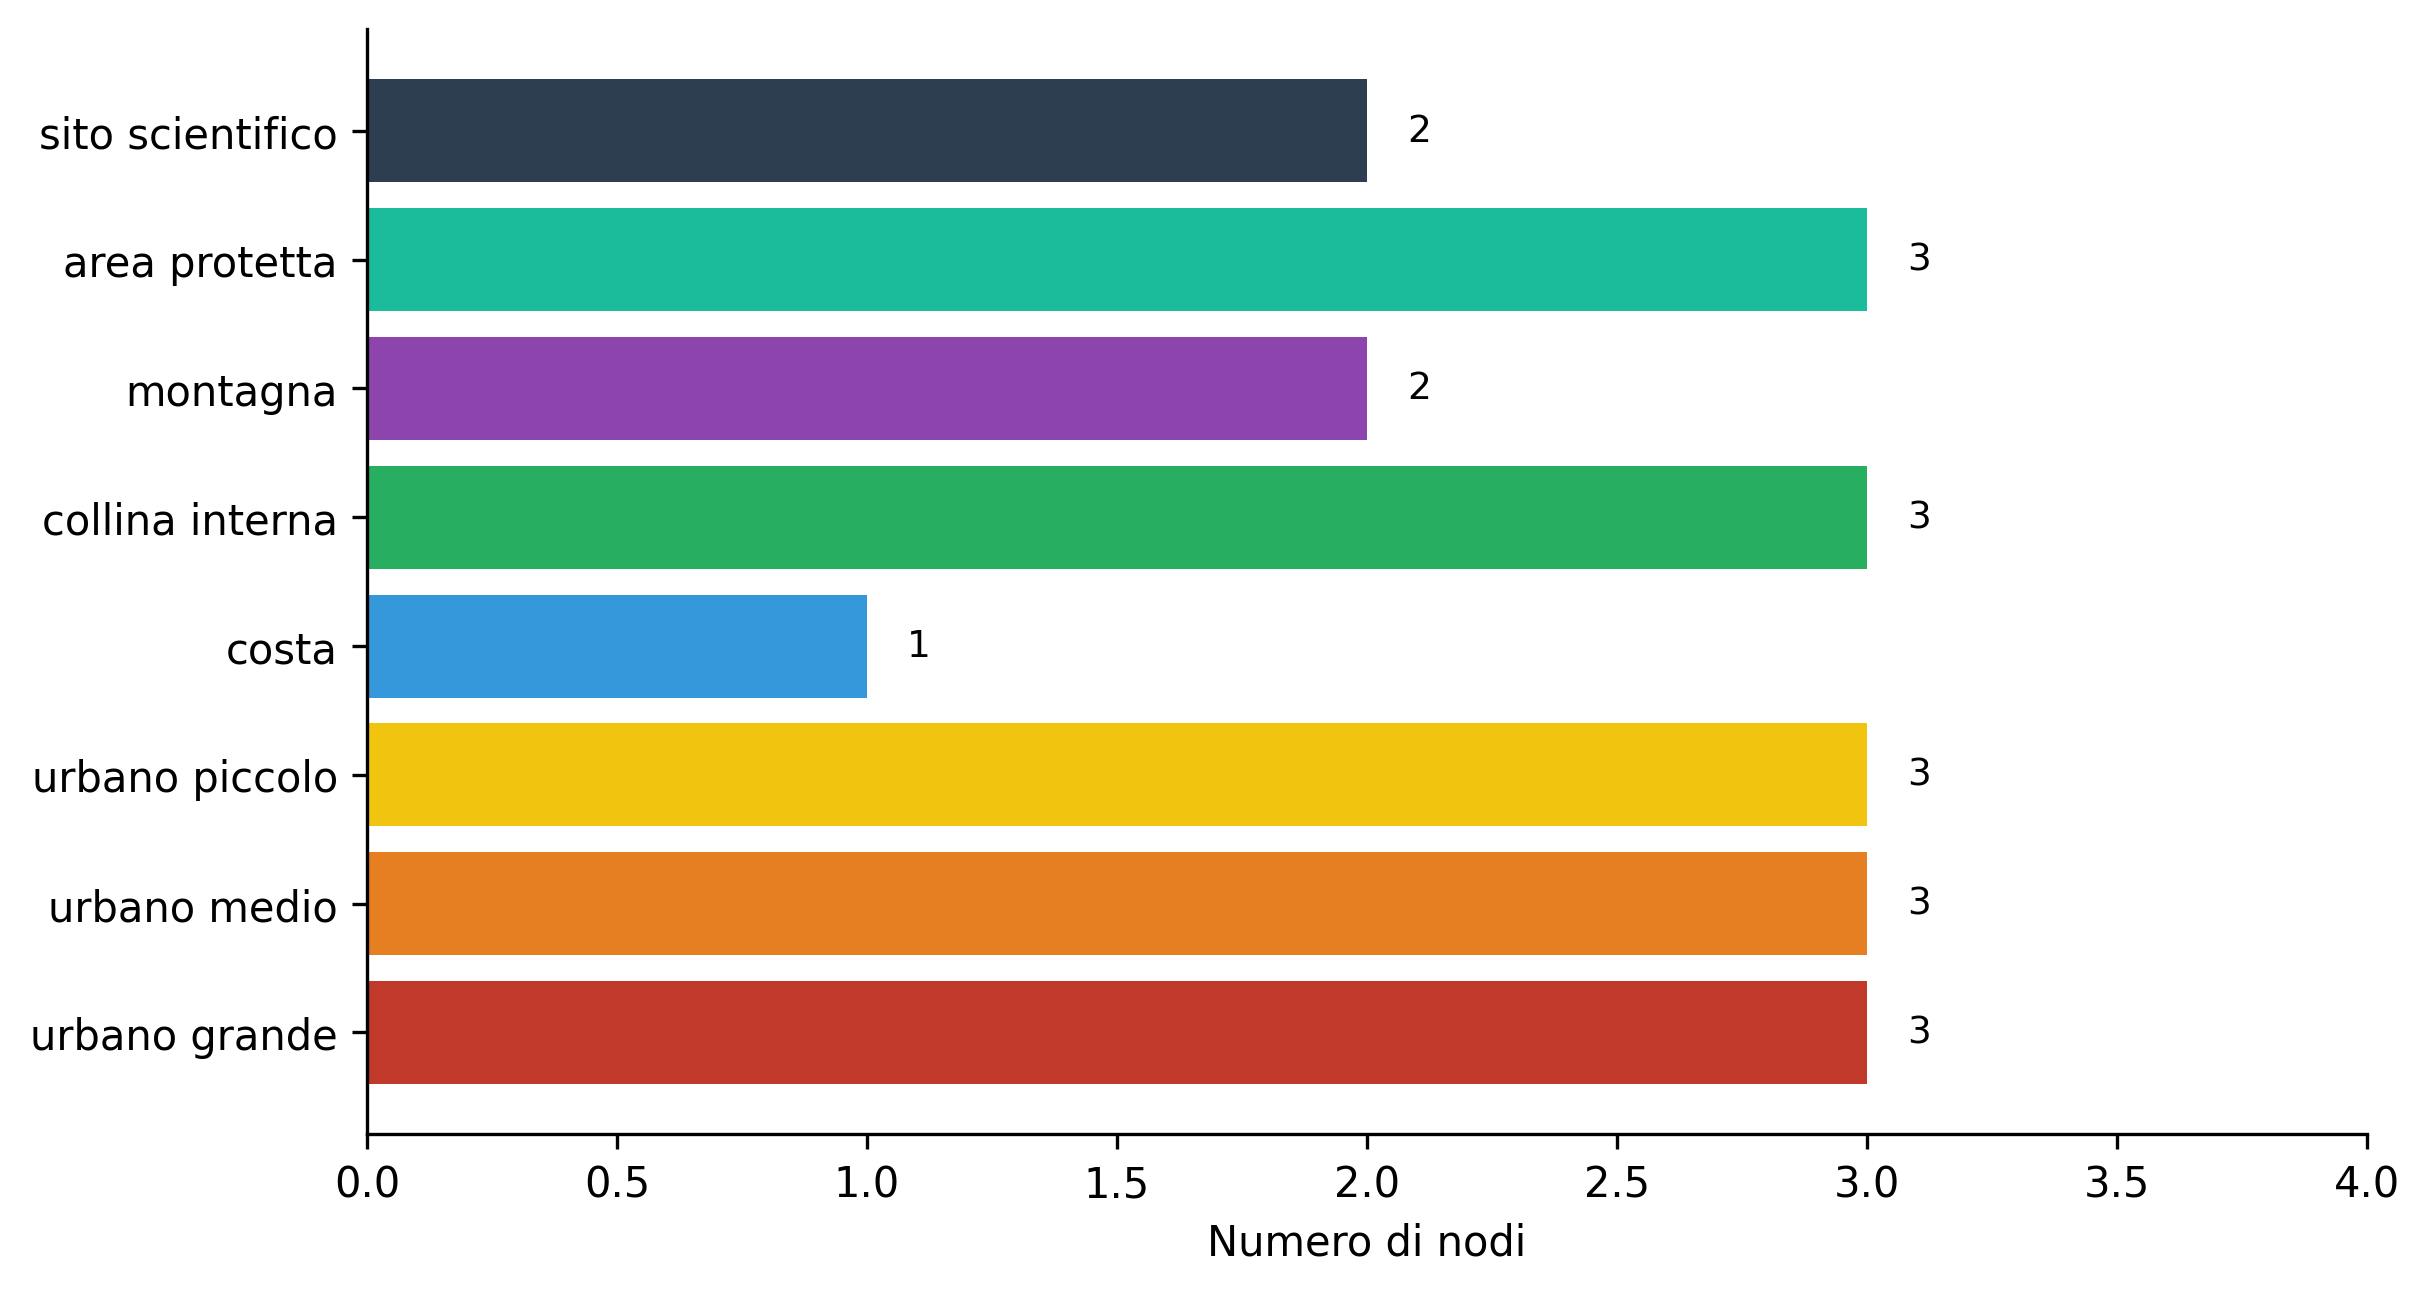
\includegraphics[width=0.95\textwidth]{figures/categorie_nodi.png}
\caption{Numero di nodi per categoria territoriale.}
\label{fig:categorie}
\end{figure}

\begin{figure}[ht!]
\centering
% Figura: scripts/generate_province.py (repo tess4c-figure-scripts). Dati: data/sites.json, campo prov.
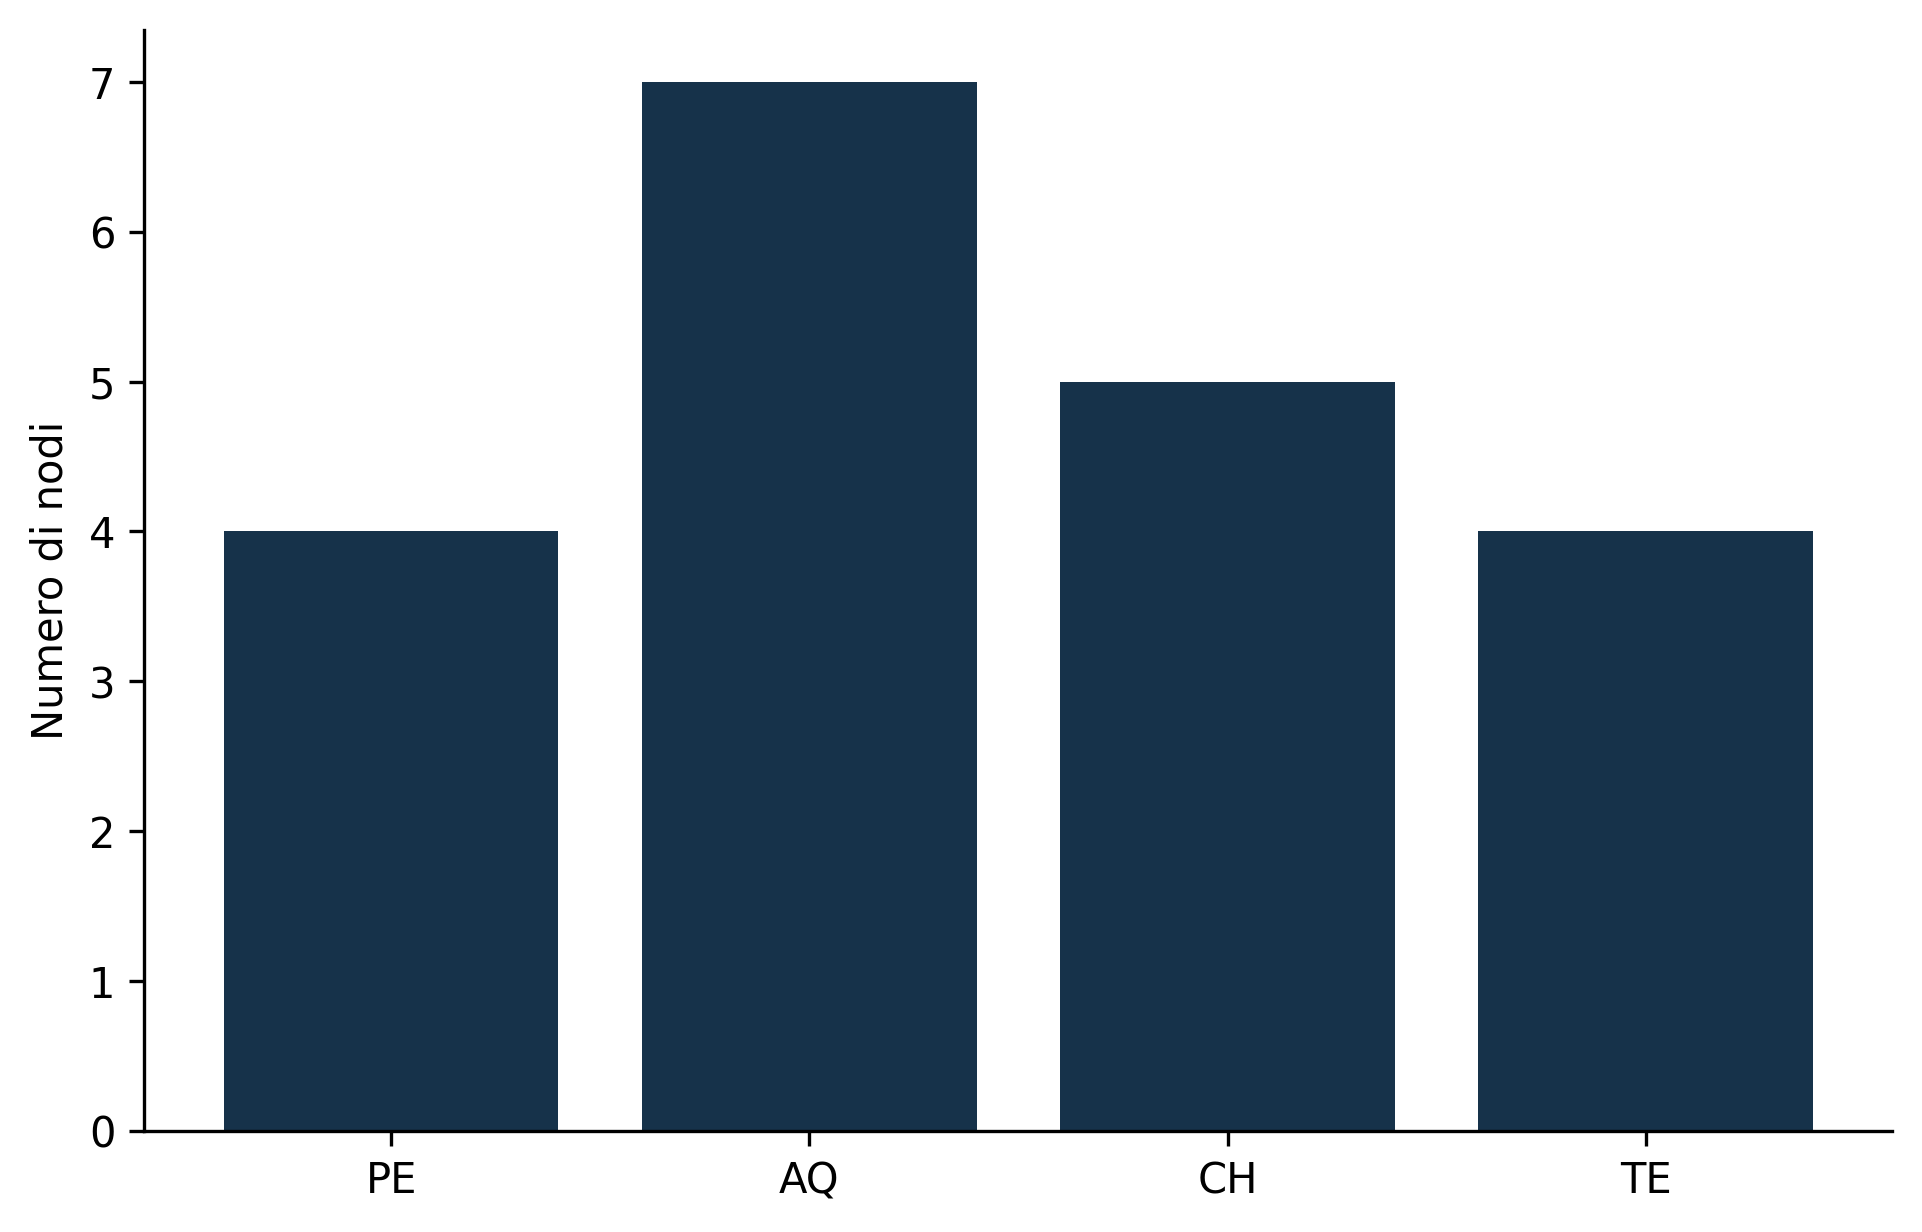
\includegraphics[width=0.78\textwidth]{figures/nodi_province.png}
\caption{Numero di nodi per provincia.}
\label{fig:province}
\end{figure}

Le 4 province sono coperte così: AQ, nodi 2, 3, 4, 9, 16, 18, 19; TE, nodi 6, 8, 15, 20; PE, nodi 1, 12, 13, 17; CH, nodi 5, 7, 10, 11, 14. I 3 parchi nazionali sono rappresentati: Gran Sasso e Monti della Laga (n.~9, 15, 19), Maiella (n.~14, 17), Abruzzo, Lazio e Molise (n.~16, 18).

\section*{Intervallo di radianza}
\addcontentsline{toc}{section}{Intervallo di radianza}

La Figura~\ref{fig:radianza} ordina i 20 nodi per radianza \textit{VIIRS} 2025 decrescente. Il massimo della rete è 95,360 nW\,cm$^{-2}$\,sr$^{-1}$ a Piazza del Duomo, L'Aquila. Il valore 2 è 94,044 a Pescara centro. Il valore 3 è 75,646 a Vasto. Il minimo è 0,000, sotto la soglia NASA 0,5, al Rifugio Bruno Pomilio (1.894\,m) e alla Stazione osservativa di Campo Imperatore (2.147\,m).

\begin{figure}[ht!]
\centering
% Figura: scripts/generate_radianza.py (repo tess4c-figure-scripts). Dati: data/sites.json, campo viirs.
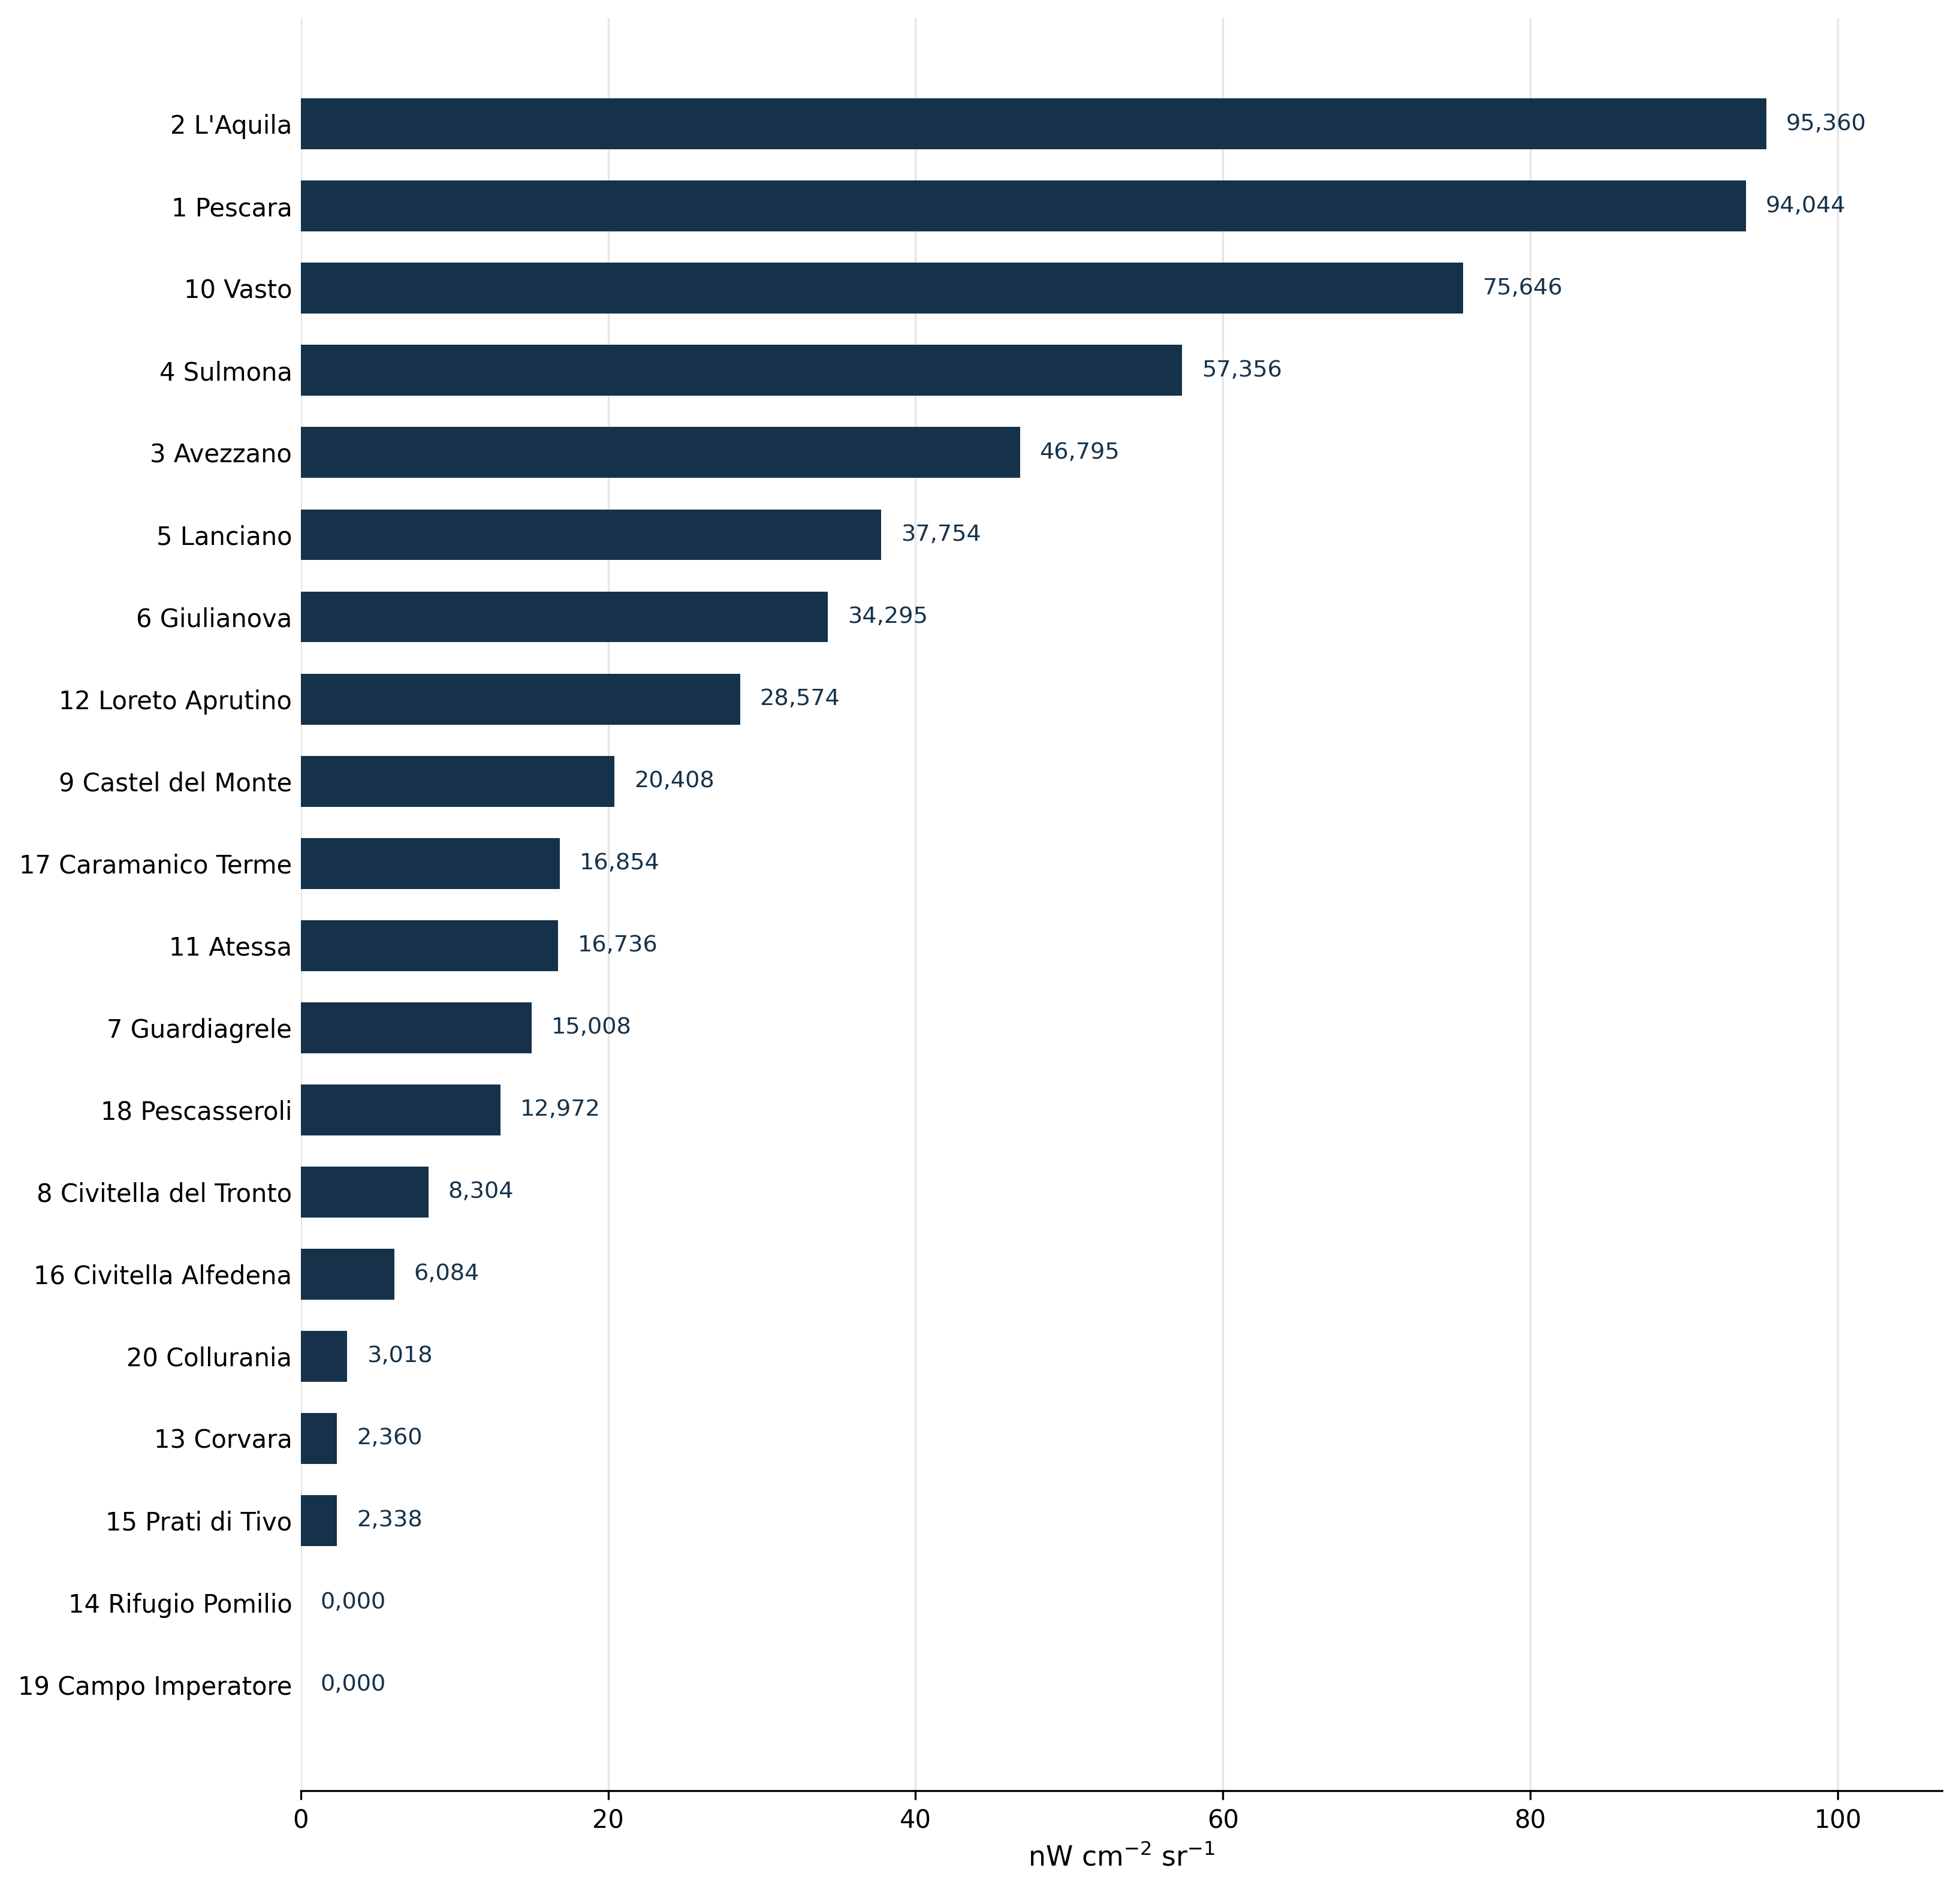
\includegraphics[height=0.48\textheight,keepaspectratio]{figures/radianza_viirs_2025.png}
\caption{Radianza VIIRS 2025 dei 20 siti candidati, in nW\,cm$^{-2}$\,sr$^{-1}$.}
\label{fig:radianza}
\end{figure}

La Figura~\ref{fig:quota} mette in relazione radianza e quota. I siti di alta quota tendono al minimo satellitare; i centri urbani restano alti anche quando non sono al livello del mare (L'Aquila). I numeri sui punti coincidono con la colonna n.\ delle tabelle.

\begin{figure}[ht!]
\centering
% Figura: scripts/generate_quota_scatter.py (repo tess4c-figure-scripts). Dati: data/sites.json, campi quota e viirs.
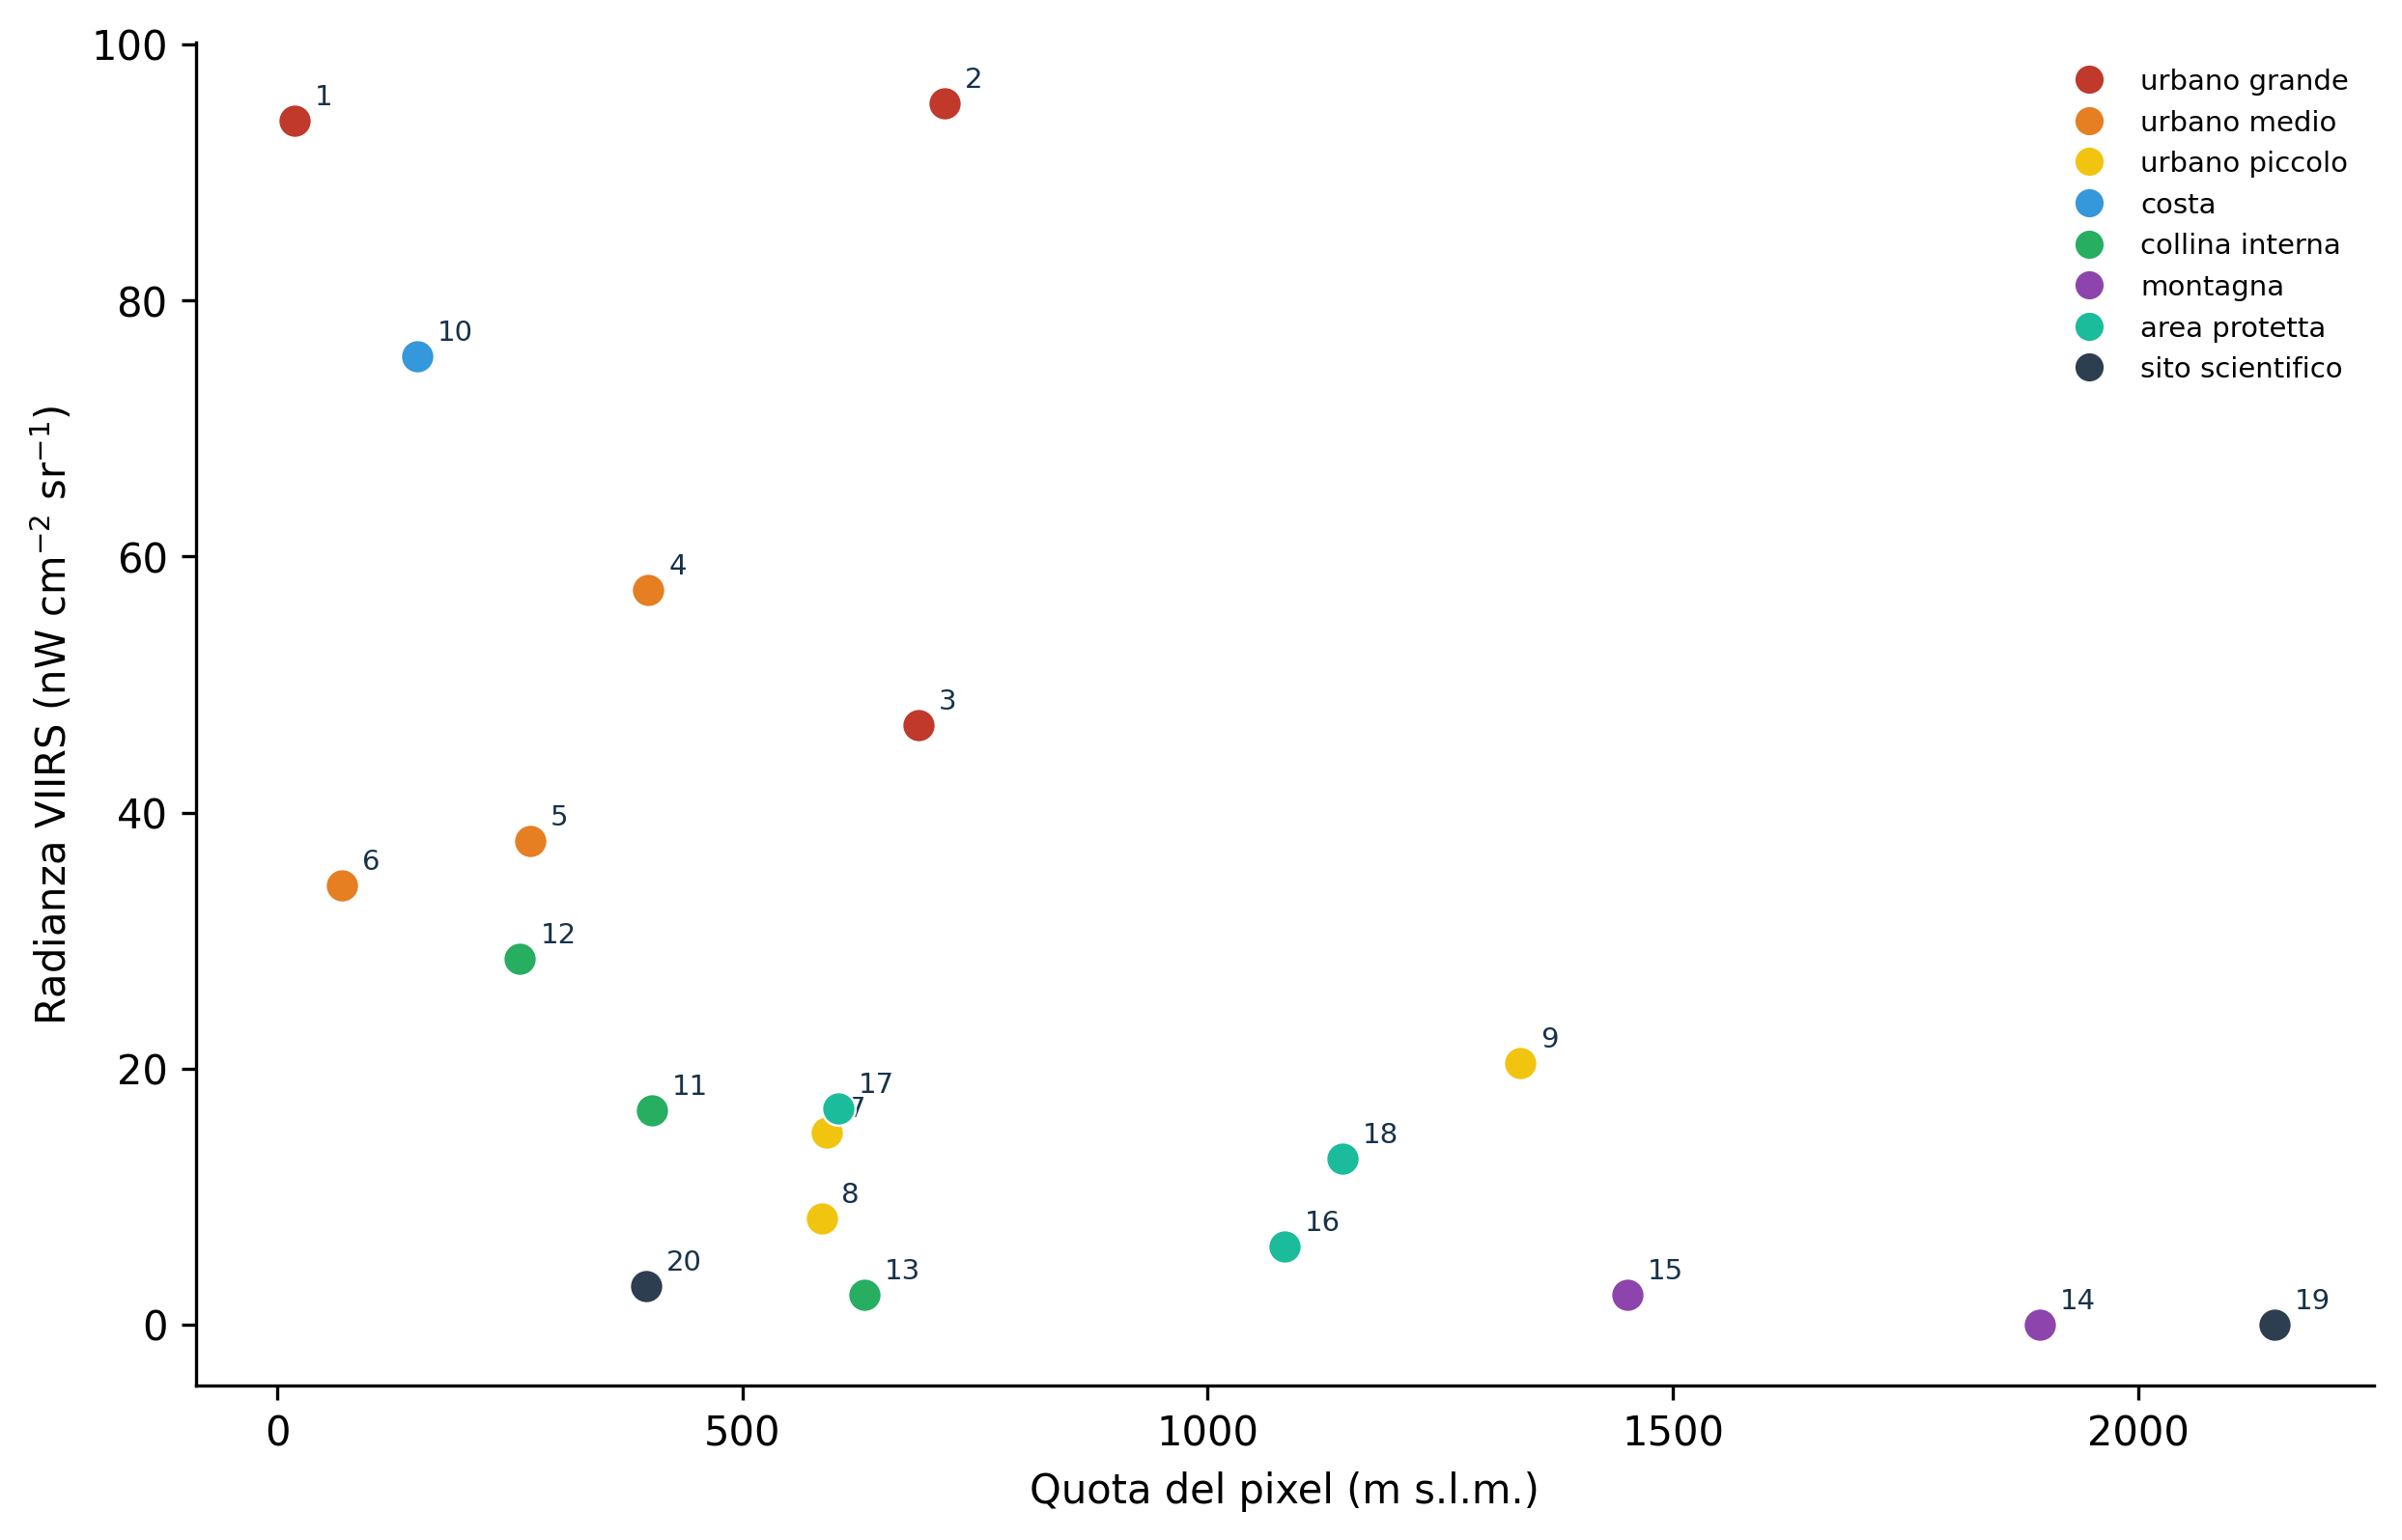
\includegraphics[width=0.95\textwidth]{figures/quota_vs_radianza.png}
\caption{Radianza VIIRS 2025 in funzione della quota del pixel. I colori indicano la categoria territoriale.}
\label{fig:quota}
\end{figure}

\FloatBarrier

\section*{Fonti}
\addcontentsline{toc}{section}{Fonti}

Le letture di radianza provengono da \url{https://www.lightpollutionmap.info/}, strato \textit{VIIRS} 2025 (NASA Black Marble VJ146A4). La documentazione del servizio (pagina di help dello stesso sito, aggiornata al 30 giugno 2026) indica unità, soglia 0,5 nW\,cm$^{-2}$\,sr$^{-1}$ e quota Copernicus WorldDEM-30.

Le popolazioni comunali al 1 gennaio 2026 sono Istat, consultate tramite Tuttitalia per le province di Pescara, L'Aquila, Teramo e Chieti.

Le coordinate derivano dalle voci Wikipedia italiane di Pescara; Piazza del Duomo (L'Aquila); Avezzano; Sulmona; Lanciano; Giulianova; Guardiagrele; Civitella del Tronto; Castel del Monte (comune); Vasto; Loreto Aprutino; Corvara (PE); Prati di Tivo; Civitella Alfedena; Pescasseroli; Rifugio Bruno Pomilio; Osservatorio astronomico di Campo Imperatore; Osservatorio astronomico d'Abruzzo. Atessa deriva dalla casa comunale Tuttitalia. Caramanico Terme deriva da OpenStreetMap.

Immagini dello strumento: GUAIX, Universidad Complutense de Madrid / STARS4ALL.

\end{document}
